\section{Results on ECUs}

This section shows and discusses the results of the implementations explained earlier.

\subsection{Coverages and request savings}

First, the coverages and request savings are assessed for each approach.

\subsubsection{Reusing information within the same service}

% RC service

\begin{table}[h]
    \begin{center}
    \begin{tabular}{ccc}
        \hline
        & \textbf{Coverage} & \textbf{Request saving} \\
        \hline
        \textbf{audi\_cgw} & 87.6\% & 65.4\% \\
        \textbf{bfft-ecu} & 100\% & 66.2\% \\
        \textbf{bmw-gateway-ecu-bdc} & 100\% & 66.2\% \\
        \textbf{bmw-gateway-ecu-zgw} & 100\% & 64.5\% \\
        \textbf{bmw-gateway-ecu2} & 100\% & 64.6\% \\
        \textbf{bmw-tcu} & 100\% & 66.7\% \\
        \textbf{bosch-ecu} & 100\% & 64.6\% \\
        \textbf{dashboard} & 50.0\% & 66.2\% \\
        \textbf{mercedes-ezs} & 100\% & 65.1\% \\
        \textbf{seppmed} & 100\% & 66.2\% \\
        \textbf{tesla-airbag-ecu} & 100\% & 66.7\% \\
        \hline

    \end{tabular}
    \end{center}
    \caption{Measured coverages and request savings on ECUs with approach 1 for the RC service.}
    \label{tab:evaluation-approach1}
\end{table}

9 of 11 ECUs had a full coverage. The coverage for the dashboard ECU notable low. Therefore, a closer look was taken there. It turned out that the Dashboard only supports two identifiers. The identifier 515 for Type1 and identifier 61,728 for Type3. The former is detected, but the resulting range for Type3 is far from the identifier 61,728. Hence, the loss and a coverage of 50\%.

For each ECU the request saving is close to the theoretical maximum of $66.7$ \%. It is so high because ECUs usually support only a few routines (see \autoref{fig:rc-distribution}). Hence, only a few identifiers are expanded to blocks and lead to more requests.

This approach is applicable to scans of services with multiple parameters. This results in a high scan time for this service and thus a high time-saving potential. However, if an identifier is not recognized during the first scan, it will not be recognized in the next scans as well.


\subsubsection{Using probabilities of positive answers based on blocks}

\begin{table}[h]
    \begin{center}
    \begin{tabular}{ccc}
        \hline
        & \textbf{Coverage} & \textbf{Request saving} \\
        \hline
        \textbf{audi\_cgw} & 87.8\% & 85.0\% \\
        \textbf{bfft-ecu} & 88.4\% & 96.6\% \\
        \textbf{bmw-gateway-ecu-bdc} & 100\% & 96.1\% \\
        \textbf{bmw-gateway-ecu-zgw} & 94.3\% & 95.8\% \\
        \textbf{bmw-gateway-ecu2} & 83.3\% & 96.1\% \\
        \textbf{bmw-tcu} & 72.2\% & 96.3\% \\
        \textbf{bosch-ecu} & 90.7\% & 93.3\% \\
        \textbf{dashboard} & 92.4\% & 94.4\% \\
        \textbf{mercedes-ezs} & 89.3\% & 94.7\% \\
        \textbf{seppmed} & 83.0\% & 95.9\% \\
        \textbf{tesla-airbag-ecu} & 100\% & 96.4\% \\
        \hline
    \end{tabular}
    \end{center}
    \caption{Measured coverages and request savings on ECUs with approach 2 for the RDBI service.}
    \label{tab:evaluation-approach2}
\end{table}

\autoref{tab:evaluation-approach2} shows the resulting coverage and request savings for this approach for the RDBI service. It should be noted, that these values vary slightly for each run because a random scan is used.

Overall, the coverages are lower with this approach than for approach 1. Only for two ECUs a coverage of 100\% is reached. The request savings are high at approximately 95\%. Nevertheless, the time savings of approach 1 are higher in practice, because that approach can be applied to larger service scans, and then a saving of about 66\% saves more time there than 95\% here.

The biggest problem with this approach is the newly added random factor. The coverage can be great for one scan, but low for the next one. This would require performing multiple scans using the new implementation to ensure that most identifiers were found.

\subsubsection{Not scanning unsupported services}

\autoref{fig:serviceNotSupported-savings} illustrates the number of saved packets for each ECU with this approach. It is only an approximation because for this graph, the responses with the both described NRCs have been counted. But actually, not every request can be saved with this approach, since at least one request must first be made to detect that this service is not supported. But this number of requests is low and negligible, especially considering that the minimum value of saved requests is about 70,000.

\begin{figure}[h]
    \centering
    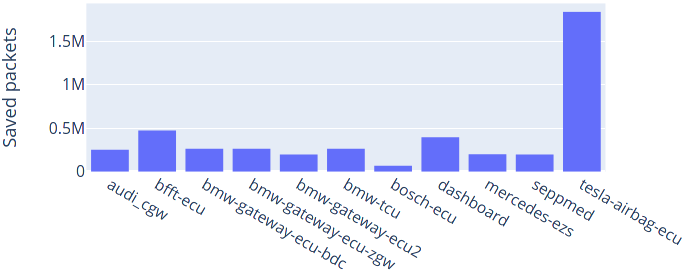
\includegraphics[width=0.8\textwidth]{serviceNotSupported-savings}
    \caption{Saved number of requests with this approach (approx).}
    \label{fig:serviceNotSupported-savings}
\end{figure}

There is a potential problem with this approach. Reliance is placed on the manufacturer to properly implement these NRCs. It is conceivable that the ECU responds to an identifier with 0x11 or 0x7f, although a subsequent identifier would actually have been answered positively. The occurrences of this behavior are shown in \autoref{fig:serviceNotSupported-losses}. It was calculated by evaluating the responses for each enumerator for each state. Once a negative response with NRC 0x11 or 0x7f was received, an internal counter was incremented with each subsequent positive response.
And in comparison to the potential savings (\autoref{fig:serviceNotSupported-savings}), the losses are negligible.

\begin{figure}[h]
    \centering
    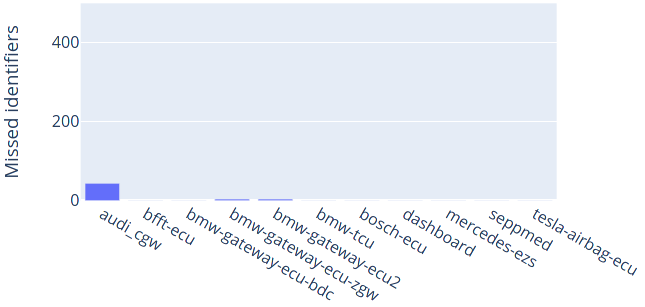
\includegraphics[width=0.8\textwidth]{serviceNotSupported-losses}
    \caption{Lost number of positive responses with this approach.}
    \label{fig:serviceNotSupported-losses}
\end{figure}

Skipping unsupported services is the safest way to save time of all three approaches. It is unlikely that identifiers will be missed, but the speed gain can still be high.

\subsection{Actual time savings}

For each ECU, the same scans were executed again as in the introduction (\autoref{sec:introduction}), they differ only in the use of the new implementations.

\begin{figure}[h]
    \centering
    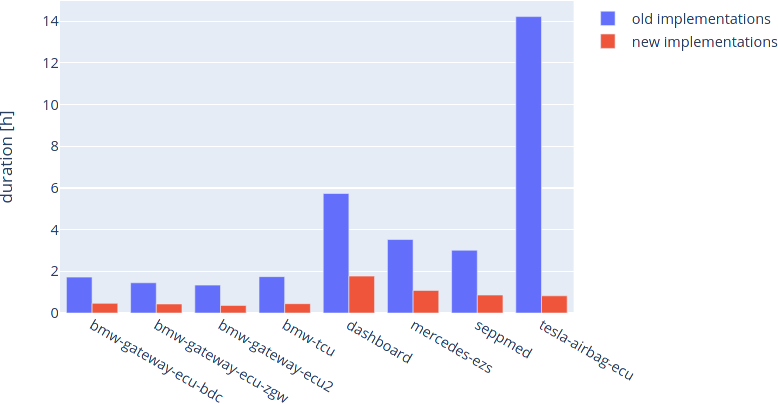
\includegraphics[width=1\textwidth]{durations-diff}
    \caption{Side by side illustration of runtimes of a UDS scan with old and new implementations.}
    \label{fig:durations-diff}
\end{figure}

As \autoref{fig:durations-diff} shows, the durations decreased significantly, especially for the Tesla ECU, which has a relatively high average response time (about 20 ms) compared to the others (1 – 8 ms).
Three ECUs are excluded from this observation because they were no longer available at the time of re-evaluating the scan durations.
